\section{Variational principle}\label{var_prin}

Here we consider the more general equation of state for the gas with
$P = K \rhog^{\Gamma}$ where $K$ is a prescribed function of position
and $\Gamma$ is a constant. The effective energy equation is then
Eq. \ref{poly_energy}. We also include the self-gravitational
potential $\psi$ of the gas
plus dust mixture, which satisfies 
%\begin{align}
$  \nabla^2 \psi  = 4 \pi G \rho. $
%\end{align} 
The linearized equations for axisymmetric
disturbances are  

\begin{align}
  \ii\sigma\frac{\delta\rho}{\rho} &= \nabla\cdot\dd\bm{v} +
  \dd\bm{v}\cdot\nabla\ln{\rho},\label{lin_mass_full}\\
%  \ii\sigma\frac{\delta P}{P} &= \nabla\cdot\dd\bm{v} +
   \ii\sigma\frac{\delta P}{P} &= \Gamma \nabla\cdot\dd\bm{v} +
  \dd\bm{v}\cdot\nabla\ln{P} - \dd\bm{v}\cdot\nabla\ln{c_s^2} - \frac{\dd\mathcal{C}}{P}.\label{lin_energy_full}\\
  -\ii\sigma\dd v_r  &= 2\Omega\dd v_\phi + 
  \hat{\bm{r}} \cdot \delta\bm{F} -  \hat{\bm{r}} \cdot \nabla\dd\psi ,\\
  \ii\sigma\dd v_\phi &= \frac{\kappa^2}{2\Omega}\dd v_r + \frac{\p
    v_\phi}{\p z}\dd v_z,\\
  -\ii\sigma\dd v_z &=  \hat{\bm{z}} \cdot \delta\bm{F}  -  \hat{\bm{z}} \cdot \nabla\dd\psi, \\ 
\nabla^2 \delta\psi & = 4\pi G \dd\rho. 
\end{align}  
where the linearizd pressure force $\delta \bm{F}$ is given in
Appendix \ref{lin_press}. These equations do not assume the
radially-local approximation used in the main text. From the
linearized meridional momentum equations, we find  

\begin{align}
  \sigma^2\int\rho\left(|\dd v_r|^2 + |\dd v_z|^2\right)dV = \int\left( \rho
  \kappa^2 |\dd v_r|^2 + \rho r\frac{\p \Omega^2}{\p z} \dd v_z \dd
  v_r^*  + \ii\sigma \rho \dd \bm{F}\cdot\dd\bm{v}^*
  - \ii \sigma \rho \nabla\dd\psi\cdot  \dd\bm{v}^* 
  \right)dV,\label{meridional}
\end{align}
where the integral is taken over the volume of the fluid. Integrating
by parts and ignoring surface integrals, the last term is
\begin{align}
  \int \ii\sigma\rho \dd \bm{F}\cdot\dd\bm{v}^*dV &=\int\left( \ii\sigma \frac{\dd
    \rho}{\rho}\dd\bm{v}^*\cdot \nabla P - \ii\sigma \dd
  \bm{v}^*\cdot\nabla \dd P  \right)dV\notag\\
&= \int\left( \ii\sigma \frac{\dd
    \rho}{\rho}\dd\bm{v}^*\cdot\nabla P + \ii\sigma \dd
 P  \nabla\cdot \dd \bm{v}^*  \right)dV\notag\\
 & = \int\left[
%   \left(
%   \ii\sigma \frac{\dd P}{P} - \dd\bm{v}\cdot\nabla s + \dd
%   \bm{v} \cdot \nabla \ln{c_s^2} + \frac{\dd\mathcal{C}}{P}
%   \right)\dd\bm{v}^*\cdot\nabla P  
   \left(
   \ii\sigma \frac{\dd P}{\Gamma P} - \dd\bm{v}\cdot\nabla \seff + \frac{\dd
   \bm{v}}{\Gamma} \cdot \nabla \ln{K} +
   \frac{\dd\mathcal{C}}{\Gamma P} \right)\dd\bm{v}^*\cdot\nabla P
   + \ii\sigma \dd P  \nabla\cdot \dd \bm{v}^*
   \right]dV\notag\\
 & = \int\left[
%   \ii\sigma\frac{\dd P}{P}\nabla\cdot\left(P\dd\bm{v}^*\right) +
%   \left(\dd\bm{v}^*\cdot\nabla P\right) \left(\dd\bm{v} \cdot \nabla
%   \ln{c_s^2} + \frac{\dd\mathcal{C}}{P}   -  \dd\bm{v}\cdot\nabla s\right) 
%   \right]dV\notag\\
   \ii\sigma\frac{\dd P}{\Gamma P}\left(\dd\bm{v}^*\cdot\nabla P +
   \Gamma P\nabla\cdot\dd\bm{v}^*   \right)
   +\left(\dd\bm{v}^*\cdot\nabla P\right) \left( \frac{\dd\bm{v}}{\Gamma} \cdot \nabla
   \ln{K} + \frac{\dd\mathcal{C}}{\Gamma P}   -  \dd\bm{v}\cdot\nabla \seff\right) 
   \right]dV\notag\\
 & = \int\left\{
%   \left[\frac{1}{P}\nabla\cdot\left(P\dd\bm{v}\right) -
%   \dd\bm{v}\cdot\nabla\ln{c_s^2} - \frac{\dd\mathcal{C}}{P}  \right]\nabla\cdot\left(P\dd\bm{v}^*\right)
%   +\left(\dd\bm{v}^*\cdot\nabla P\right)\left(\dd\bm{v} \cdot \nabla
%   \ln{c_s^2} + \frac{\dd\mathcal{C}}{P}   -  \dd\bm{v}\cdot\nabla s \right)
%   \right\}dV \notag\\
 \left[
   \nabla\cdot\dd\bm{v} +
  \frac{\dd\bm{v}}{\Gamma}\cdot\nabla\ln{P} -
  \frac{\dd\bm{v}}{\Gamma}\cdot\nabla\ln{K} -
  \frac{\dd\mathcal{C}}{\Gamma P}. 
  \right]
 \left(\dd \bm{v}^*\cdot\nabla P +
 \Gamma P\nabla\cdot\dd\bm{v}^*   \right)\right. \notag\\
 &\phantom{=\int\left\{\right\}}\left. 
 + \left(\dd\bm{v}^*\cdot\nabla P\right)\left(\frac{\dd\bm{v}}{\Gamma} \cdot \nabla
 \ln{K}
 + \frac{\dd\mathcal{C}}{\Gamma P}   -  \dd\bm{v}\cdot\nabla \seff \right)
 \right\}dV \notag\\
 &=\int\left[
%     \frac{1}{P}\left|\nabla\cdot\left(P\dd\bm{v}\right)\right|^2 -
%     \left(\dd\bm{v}^*\cdot\nabla P\right)\left(\dd\bm{v}\cdot\nabla s
%     \right) -
%     P\left(\nabla\cdot\dd\bm{v}^*\right)\left(\dd\bm{v}\cdot\nabla\ln{c_s^2} + \frac{\dd\mathcal{C}}{P} \right)  
    \frac{1}{\Gamma P} \Bigl\lvert \dd \bm{v}\cdot\nabla P +
 \Gamma P\nabla\cdot\dd \bm{v}    \Bigr\rvert ^2 - 
     \left(\dd\bm{v}^*\cdot\nabla P\right)\left(\dd\bm{v}\cdot\nabla \seff
     \right) -
      P\left(\nabla\cdot\dd\bm{v}^*\right)\left(\dd\bm{v}\cdot\nabla\ln{K} + \frac{\dd\mathcal{C}}{P} \right) 
     \right]dV,
\end{align}
where  $\seff\equiv\ln{(P^{1/\Gamma}/\rho)}$. 
The self-gravitational part of Eq. \ref{meridional} is, again
nelgecting surface terms when integrating by parts, 
\begin{align}
-\int \ii\sigma \rho \nabla\dd\psi \cdot\dd  \bm{v}^* &= \int \ii\sigma
  \dd\psi \nabla\cdot\left(\rho\dd\bm{v}^*\right) dV
 = \int \left|\sigma\right|^2 \dd\psi \dd \rho^*dV 
  = -\frac{1}{4\pi G}\int   \left|\sigma\right|^2
   \left|\nabla\psi\right|^2 dV,  
\end{align}
where the linearized continuity and Poisson equations have been used. 

Hence,
\begin{align}\label{integral_ex}
  &\sigma^2\int\rho\left(|\dd v_r|^2 + |\dd v_z|^2\right)dV \notag\\
&=  \int\left\{
  \rho |\dd v_r|^2 \left(\kappa^2 - \frac{1}{\rho}\frac{\p P}{\p
    r}\frac{\p \seff}{\p r}\right)
  + \rho |\dd v_z|^2\left(-\frac{1}{\rho}\frac{\p P}{\p
    z}\frac{\p \seff}{\p z}\right)
   + \rho \dd v_z \dd v_r^*\left(r\frac{\p\Omega^2}{\p z} -
  \frac{1}{\rho}\frac{\p P}{\p
    r}\frac{\p \seff}{\p z}\right) 
  + \rho \dd v_z^*\dd v_r \left(-\frac{1}{\rho}\frac{\p P}{\p
    z}\frac{\p \seff}{\p r}\right)\right. \notag\\
&\phantom{==\int}\left.+
%  \frac{1}{P}\left|\nabla\cdot\left(P\dd\bm{v}\right)\right|^2
 \frac{1}{\Gamma P}\Bigl\lvert \dd\bm{v}\cdot\nabla P +
 \Gamma P\nabla\cdot\dd\bm{v}     \Bigr\rvert^2
 - \frac{1}{4\pi G}\left|\sigma\nabla\dd\psi\right|^2 
  \right\}dV 
%  P\left(\nabla\cdot\dd\bm{v}^*\right)\left(\dd\bm{v}\cdot\nabla\ln{c_s^2}\right)dV
-\int    P\left(\nabla\cdot\dd\bm{v}^*\right)\left(\dd\bm{v}\cdot\nabla\ln{K}\right)dV
  -\int \left(\nabla\cdot\dd\bm{v}^*\right)\dd\mathcal{C}dV.  
\end{align}
Note that the coefficient of $\delta v_z\delta v_r^*$ and $\delta
v_z^*\delta v_r$ are equal owing to the equilibrium state
(Eq. \ref{vshear}). The non-self-gravitating case with $\Gamma=1,\, K = c_s^2$ gives
Eq. \ref{int_rel}. Similar integral relations are given by 
\cite{kato78, kley93,latter06}.  

%If $c_s$ is constant then the second integral vanishes, $\sigma^2$
%is real, and the first integral leads to the usual Solberg-Hoiland
%criteria. However, for a stationary but non-uniform temperature
%profile, the second  

\section{Linearized pressure forces and its divergence}\label{lin_press}
%Define
%\begin{align}
 % \bm{F} \equiv - \frac{\nabla P}{\rho}. 
%\end{align}
The linearized form of the pressure force $\bm{F} = -\nabla P/\rho$ is  
\begin{align}
  \delta \bm{F} = - \frac{\dd\rho}{\rho}\bm{F} -
  \frac{1}{\rho}\nabla\dd P,
\end{align}
with divergence
\begin{align}
  \nabla\cdot\dd\bm{F} = -
  \nabla\left(\frac{\dd\rho}{\rho}\right)\cdot\bm{F} -
  \frac{\dd\rho}{\rho}\nabla\cdot\bm{F} +
  \nabla\ln{\rho}\cdot\frac{\nabla\dd P}{\rho} -
  \frac{1}{\rho}\nabla^2\dd P. 
\end{align}

%\subsection{Explicit expressions}

The explicit forms for $\dd\bm{F}$ and $\nabla\cdot\dd\bm{F}$, in the
radially-local approximation, are
\begin{align}
  &\dd F_r = - W F_r - \ii k_x Q,\\
  &\dd F_z = - W F_z - \left[Q^\prime + Q
    \left(\ln{\rho}\right)^\prime\right]  = - \ii\sigma \dd v_z, 
\end{align} 
where the last equality is the linearized
vertical momentum equation; and 
\begin{align}
  \nabla\cdot\dd\bm{F} &= F_r\left(\p_r\ln{\rho} - \ii k_x \right)W - F_z
  W^\prime - W \nabla\cdot\bm{F} + \ii k_x Q \p_r\ln{\rho} +
  \left(\ln{\rho}\right)^\prime\left[Q^\prime + Q
    \left(\ln{\rho}\right)^\prime\right] \notag\\
  & \phantom{=} + k_x^2 Q - \left\{Q^{\prime\prime} + 2
    Q^\prime\left(\ln{\rho}\right)^\prime
    + Q\left[\left(\ln{\rho}\right)^{\prime\prime}+\left(\ln{\rho}\right)^{\prime
      2}\right]\right\}\notag\\
    &= \left[\left(\p_r\ln{\rho}-\ii k_x\right)F_r - \nabla\cdot\bm{F} +
      F_z^\prime\right]W + \left(\ii k_x \p_r\ln{\rho} + k_x^2\right)Q  -
      \ii\sigma \dd v_z^\prime.
\end{align}




\section{Linearized dust diffusion}\label{lin_dust}
We consider small grains in the Epstein regime, with fixed internal
density and size, so that
\begin{align}
  \tstop  =  \frac{K}{\rho c_s}\label{epstein}
\end{align}
\citep{price15}, where $K$ is a constant. Then the dust diffusion
function becomes
\begin{align}
  \mathcal{C} \equiv c_s^2\nabla\cdot\left(\tepsilon\tstop\nabla
  P\right) = - K c_s^2 \nabla\cdot
  \left(\frac{\tepsilon}{c_s}\bm{F}\right) =
  -Kc_s \left(\bm{F}\cdot\nabla\tepsilon + \tepsilon \nabla\cdot\bm{F}
  - \frac{1}{2}\tepsilon\bm{F}\cdot\nabla\ln{c_s^2}\right).  
\end{align}
Linearizing,
\begin{align}
  - \frac{\dd\mathcal{C}}{Kc_s} = \bm{F}\cdot\nabla\dd\tepsilon +
  \dd\bm{F}\cdot\nabla\tepsilon + \dd\tepsilon\nabla\cdot\bm{F} +
  \tepsilon\nabla\cdot\dd\bm{F} -
  \frac{1}{2}\nabla\ln{c_s^2}\cdot\left(\bm{F}\dd\tepsilon + \tepsilon
  \dd\bm{F}\right). 
\end{align}
The linearized dust-fraction $\dd\tepsilon$ and its derivatives in the
radially-local approximation are given by
\begin{align}
  \dd\tepsilon      &= (1-\tepsilon)W - \frac{Q}{c_s^2}, \\
  \p_r\dd\tepsilon &= \left[(1-\tepsilon)\left(\ii k_x -
    \p_r\ln{\rho}\right) - \p_r\tepsilon\right]W + \left(\p_r\ln{c_s^2}
  + \p_r\ln{\rho} - \ii k_x \right)\frac{Q}{c_s^2},\\
  \dd\tepsilon^\prime &= (1-\tepsilon)W^\prime - \tepsilon^\prime W -
  \left(\frac{Q}{c_s^2}\right)^\prime. 
\end{align}

%\section{Conversion formulae}
%The gas density $\rhog$ and dust-to-gas ratio $\epsilon$ is related
%to the total density $\rho$ and dust-fraction $\tepsilon$ by
%\begin{align}
%  \ln{\rho} &= \ln{\rhog} + \ln{\left(1 + \epsilon\right)},\\
%  \nabla\ln{\rho} &= \nabla\ln{\rhog} + \frac{\nabla\epsilon}{1+
%    \epsilon},\\
%  \nabla^2\ln{\rho} &= \nabla^2\ln{\rhog} +
%  \frac{\nabla^2\epsilon}{1+\epsilon} -
%  \frac{\left|\nabla\epsilon\right|^2}{\left(1+\epsilon\right)^2}, 
%\end{align}
%and
%\begin{align}
%  \tepsilon &= \frac{\epsilon}{1+ \epsilon},\\
% \nabla\tepsilon & =
% \frac{\nabla\epsilon}{\left(1+\epsilon\right)^2},\\
% \nabla^2\tepsilon &=
% \frac{\nabla^2\epsilon}{\left(1+\epsilon\right)^2} -
% \frac{2\left|\nabla\epsilon\right|^2}{\left(1+\epsilon\right)^3}. 
%\end{align}

\section{One-fluid dispersion relation for the streaming instability}\label{compressible_streaming}
We consider an unstratified disk with $\Phi = \Phi (r)$ so that $\p_zP = \p_z\rho =
0$. The background $\p_rP/\rho$, $\tepsilon$ are constant
input parameters. Then for the Epstein drag law, Eq. \ref{epstein}, we
have $\mathcal{C}=0$ in the background state. 
We Fourier analyze in $r$ and $z$ so that $\p_z\to \ii k_z$ and
$\p_r\to \ii k_x$ when acting on perturbations, and denote $|\bm{k}|^2
\equiv k_x^2 + k_z^2$. We consider large $k_x$ and background
gradients when compared with that of  perturbations. 
%neglect the radial density gradient compared to that of pertuburbations 
%(formally setting $\p_r\rho=0$). 
 This is also done in most local studies of
dusty disks \citep[e.g.][]{youdin07b}.  
The linearized
equations are, after eliminating the azimuthal velocity: 

\begin{align}
  \ii \sigma W &=\nabla\cdot \dd \bm{ v} = \ii k_x \dd v_x + \ii k_z \dd v_z,\label{streaming_mass}\\
    \sigma^2 \dd v_x &= \kappa^2 \dd v_x - \ii \sigma F_r W +
    k_x\sigma Q,\label{streaming_vx}\\
  -\ii\sigma\dd v_z &= -\ii k_zQ,\label{streaming_vz}\\
\ii \zeta \sigma  Q & = \frac{P}{\rho} \nabla \cdot \dd\bm{v}   -
  \frac{\dd \mathcal{C}}{\rho}. 
\end{align}
%{\bf bg pressure gradient neglected in energy eq (is this ok? could
%  fix, but get more complicated dispersion}
The artifical factor $\zeta = 1$  is inserted to keep track of the
left-hand-side of the energy equation. We note that the incompressible
condition used by \cite{jacquet11} is obtained by setting $\zeta$ to zero. 
The linearized dust diffusion
function (Appendix \ref{lin_dust}), 
under the above approximations, is 
\begin{align}
-\frac{\dd \mathcal{C}}{\rho}  = \tstop c_s^2 \left[\ii k_x F_r\left( 1-2\tepsilon\right)
  W + \tepsilon |\bm{k}|^2 Q\right]. 
\end{align}
%{\bf only the second term contributes to work done? dont think so}

We eliminate the velocity perturbations to obtain
\begin{align}
  \left(\ii \zeta \sigma - \tstop c_s^2 \tepsilon |\bm{k}|^2\right)Q &=
  \ii \left[
  \frac{P}{\rho}\sigma + k_x\tstop c_s^2 F_r\left(1 -
  2\tepsilon\right)\right]W, \\
   \sigma^2 \left( \kappa^2 - \sigma^2 - \ii k_x F_r\right)W &=
    \left(k_z^2\kappa^2 - \sigma^2|\bm{k}|^2\right)Q, 
\end{align}
which yields the dispersion relation
\begin{align}
  &\frac{\zeta}{c_s^2|\bm{k}|^2}\sigma^5 + \ii \tepsilon \tstop
  \sigma^4 - \left[ \frac{\zeta}{c_s^2|\bm{k}|^2} \left(\kappa^2 - \ii
  k_x F_r\right) + \left(1 - \tepsilon\right)\right]\sigma^3 - \ii
  \tstop \left[\tepsilon \kappa^2 - \ii k_x F_r\left( 1 -
  \tepsilon\right)\right]\sigma^2 \notag\\ 
  &+ \left(1 -
  \tepsilon\right)\left(\frac{k_z\kappa}{|\bm{k}|}\right)^2\sigma +
  k_x \tstop F_r\left(1 - 2\tepsilon\right)
  \left(\frac{k_z\kappa}{|\bm{k}|}\right)^2  = 0.\label{streaming_dispersion}
\end{align}
The equation of state $P = c_s^2\left( 1 - \tepsilon\right)\rho$
was used.


\subsection{Incompressible limit}

 We can set $\zeta = 0$ or consider $c_s^2\to \infty$ to
obtain the incompressible limit. Using $\tau_\mathrm{s} \equiv
\tstop/\left(1 - \tepsilon\right)$, we obtain: 
\begin{align}
\ii \tepsilon \tau_\mathrm{s}
  \sigma^4 - \sigma^3 - 
  \tau_\mathrm{s} \left[ \ii \tepsilon \kappa^2 + k_x F_r\left( 1 -
  \tepsilon\right)\right]\sigma^2 
  + \left(\frac{k_z\kappa}{|\bm{k}|}\right)^2\sigma + 
  k_x \tau_\mathrm{s} F_r\left(1 - 2\tepsilon\right)
  \left(\frac{k_z\kappa}{|\bm{k}|}\right)^2  = 0,\label{streaming_incompressible}
\end{align}
as derived by \cite{jacquet11} and \cite{laibe14} for the streaming
instability. 
If $|\sigma|/\OmK = O(\tau_\mathrm{s}\OmK)$ and
$\tau_\mathrm{s}\OmK\ll 1$, then the quartic term
is small and may be neglected. In that case we obtain the cubic
dispersion relation of \citet{youdin05a}. 

\subsection{Spuriously growing epicycles}\label{spurious_epi}

A caveat of the dispersion relations 
Eq. \ref{streaming_dispersion} and \ref{streaming_incompressible} is
that they admit spurious unstable modes with $|\sigma|\gtrsim \Omega$
that violates the one-fluid framework used in this
paper. We demonstrate this below by considering the
incompressible dispersion relation. (We checked numerically that
compressibilty has negligible effects on the modes examined.) 

Consider the limit $k_z=0$. Then Eq. \ref{streaming_incompressible}
becomes 
\begin{align}      %streaming_incompressible
\ii \sigma^2 - \frac{\sigma}{\epsilon \tstop}  - \left(\ii \kappa^2 +
  \frac{k_xF_r}{\epsilon}\right) = 0. \label{kz_zero_si}
\end{align} 
Neglecting the quadratic term leads to stability, $\imag{\sigma}<0$, 
as found by \cite{youdin05a} in their full two-fluid analysis as 
$k_z\to0$.  
% However, the real and imaginary parts of Eq. \ref{kz_zero_si}  are
% \begin{align}
% \omega\left(2 s + \frac{1}{\epsilon\tstop}\right) - \frac{k_xF_r}{\epsilon} & =
%                                                                      0, \label{epi_overs1} \\
% \omega^2 - s^2 - \frac{s}{\epsilon\tstop}  - \kappa^2 &= 0, \label{epi_overs2}
% \end{align}
% so the growth rate satisfies 
% \begin{align*}
% \left( \frac{k_xF_r\tstop}{1 + 2 s\epsilon\tstop}\right)^2 - s^2
%   - \frac{s}{\epsilon \tstop} = \kappa^2. %\omega = \frac{k_xF_r\tstop}{1 + 2 s\epsilon\tstop}
% \end{align*} 
However, solving Eq. \ref{kz_zero_si} explicitly assuming $\epsilon s \tstop \ll 1$ would yield 
\begin{align}
  |\omega| &\simeq \left|k_xF_r\right| \tstop \sim \kappa, \\
  s &\simeq \epsilon \tstop \left[\left(k_xF_r\tstop\right)^2 - \kappa^2\right],\label{epi_grow}
\end{align}
Accordingly, given $k_xF_r$, growth is possible if 
\begin{align}
\tstop > \frac{\kappa}{k_x\left|F_r\right|}\equiv t_{\mathrm{s}0}.\label{epi_grow_criterion}
\end{align}
The mode is marginally stable when $\tstop =
t_{\mathrm{s}0}$. Alternatively, for fixed $\tstop$ growth is enabled
by a sufficiently large $k_xF_r$. Unlike the streaming instability,
which is strongly surpressed when $\epsilon=1$, these modes can still
grow at equal dust-to-gas ratio.  

These growing epicycles have $|\omega|\gtrsim \kappa$. 
However, these modes are absent in full two-fluid
models \citep{youdin05a}. The discrepency lies in the fact that the
first-order  one-fluid equations are only valid for low-frequency waves with
$|\sigma|\lesssim \Omega$. Thus only 
low-frequency modes should be retained from analyses based on the
first-order one-fluid approximation. 

%When this is violated,
%terms of $O(\tstop^2)$ should be retained in deriving the one-fluid
%equations (Eq. \ref{masseq}---\ref{tempeq}).  

Fig. \ref{dusty_growth1} show unstable modes found from
Eq. \ref{streaming_dispersion} as a function of $K_z$ at fixed $K_x 
= 1500$, $\epsilon=2$ and $\taus\OmK=0.01$.  
The (spurious) overstable dusty epicycles' growth
rates are weakly depedent on $K_z$ and are well approximated by
that in the $K_z=0$ limit, Eq. \ref{epi_grow}, which becomes 
\begin{align*} 
  s = \epsilon \left(1 - \tepsilon
  \right)\taus\OmK^2\left[4K_x^2\left(1-\tepsilon\right)^4\left(\taus\OmK\right)^2
  -1 \right]
\end{align*}
in the above notation. 
For the case considerd in Fig. \ref{dusty_growth1} we find
$s\simeq0.067\OmK$, as observed. By contrast, the streaming
instability requires $K_z>0$, and dominates when
$K_z\gtrsim 100$. 

\begin{figure}
  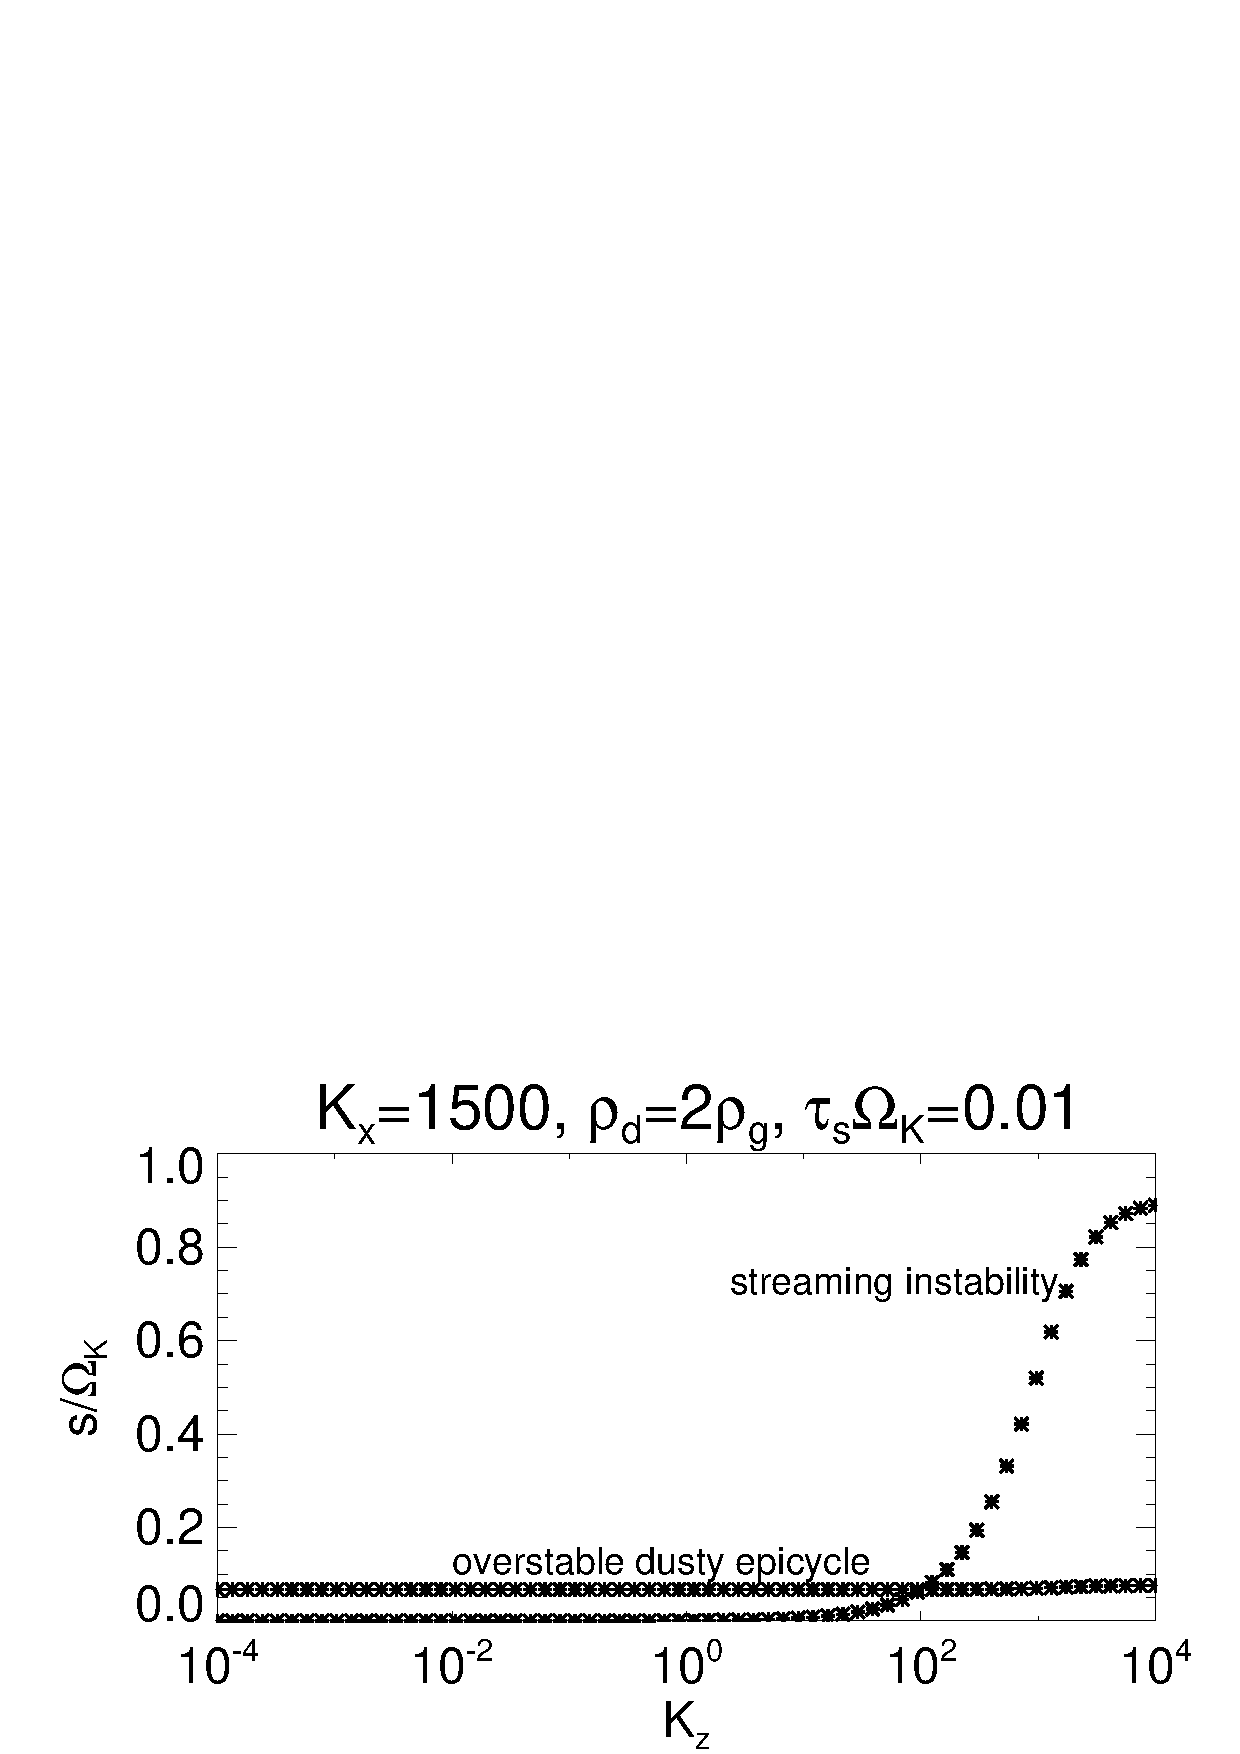
\includegraphics[width=\linewidth]{figures/streaming2}
  \caption{Growth rates of dust-drag instabilities with fixed radial
    wavenumber and dust-to-gas ratio, as a function of
    the vertical wavenumber at fix stopping time. \label{dusty_growth1}
  }
\end{figure}

Caution must be taken if the first-order one-fluid equations are used
to simulate dusty gas. 
%One should ensure that the physical dust-gas instabilty
%(which should have low-frequency in order for the first-order one-fluid
%approximation) has a larger growth rate than that of the spurious
%modes, which is given by Eq. \ref{epi_growth}. 
%Fig. \ref{dusty_growth1} suggests that the
%streaming instability would dominate, provided there is sufficient
%resolution to resolve high $K_z$ modes.  
For example, 2D, razor-thin disks would allow the spurious epicycles
to dominate, since in that case the streaming instability cannot
operate. Fig. \ref{dusty_growth1} suggest that in a realistic 3D disks
where a range of $K_z$ is allowed, the streaming instability should
dominate. 

Thus simulations based on the first-order one-fluid equations should
be set up to surpress these spurious epicycles. This might be
achieved, for example, through physical or numerical viscosity to
eliminate high-$k_x$ modes, since for fixed disk/dust parameters these
spurious epicycles only operate at sufficiently small radial
wavelengths. Alternatively, one needs to ensure the physical
instabilities of interest have larger growth rates than the spurious
epicycles. 


%An important caveat is that the one-fluid approximation for dusty gas 
%may not hold well when $|\omega| \gtrsim 
%\Omega$ \citep{youdin05a}, as is the case for dusty epicycles. 

% Their
% existence should be checked with full dust-plus-gas 
% simulations. Several 2D, razor-thin disk simulations do suggest a
% dusty instability that destory vortices
% \citep{fu14b,raettig15,surville16}. These setups are significantly
% more complex than our models, but \citeauthor{raettig15} did find 
% particle clumping in a test simulation without a vortex. These results
% might be related to the overstable dusty epicycles discussed here.       


% Real disks are three-dimensional, so the importance of dusty 
% epicycles should be compared with $k_z\neq0$ modes, which
% includes the classic streaming instability \citep{youdin05a},
% discussed next. 

%\subsection{Numerical example}


% In Fig. \ref{dusty_growth2} we fix the wavenumbers and vary the
% stopping time. The vertical dashed line is the critical stopping time
% for the overstable dusty epicycles, Eq. \ref{epi_grow_criterion},
% which is  
% \begin{align*}
%   \tau_{\mathrm{s,min}}\OmK = \frac{1}{2K_x\left(1-\tepsilon\right)^2} 
% \end{align*}
% in the above notation. For this example, $\tau_{\mathrm{s,min}}\OmK\simeq 
% 0.003$, as observed. On the other hand, the streaming instability
% shows weak dependence on $\taus$ for this range of stopping times 
% (it ultimated vanishes as $\taus\to0$). 

% \begin{figure}
%   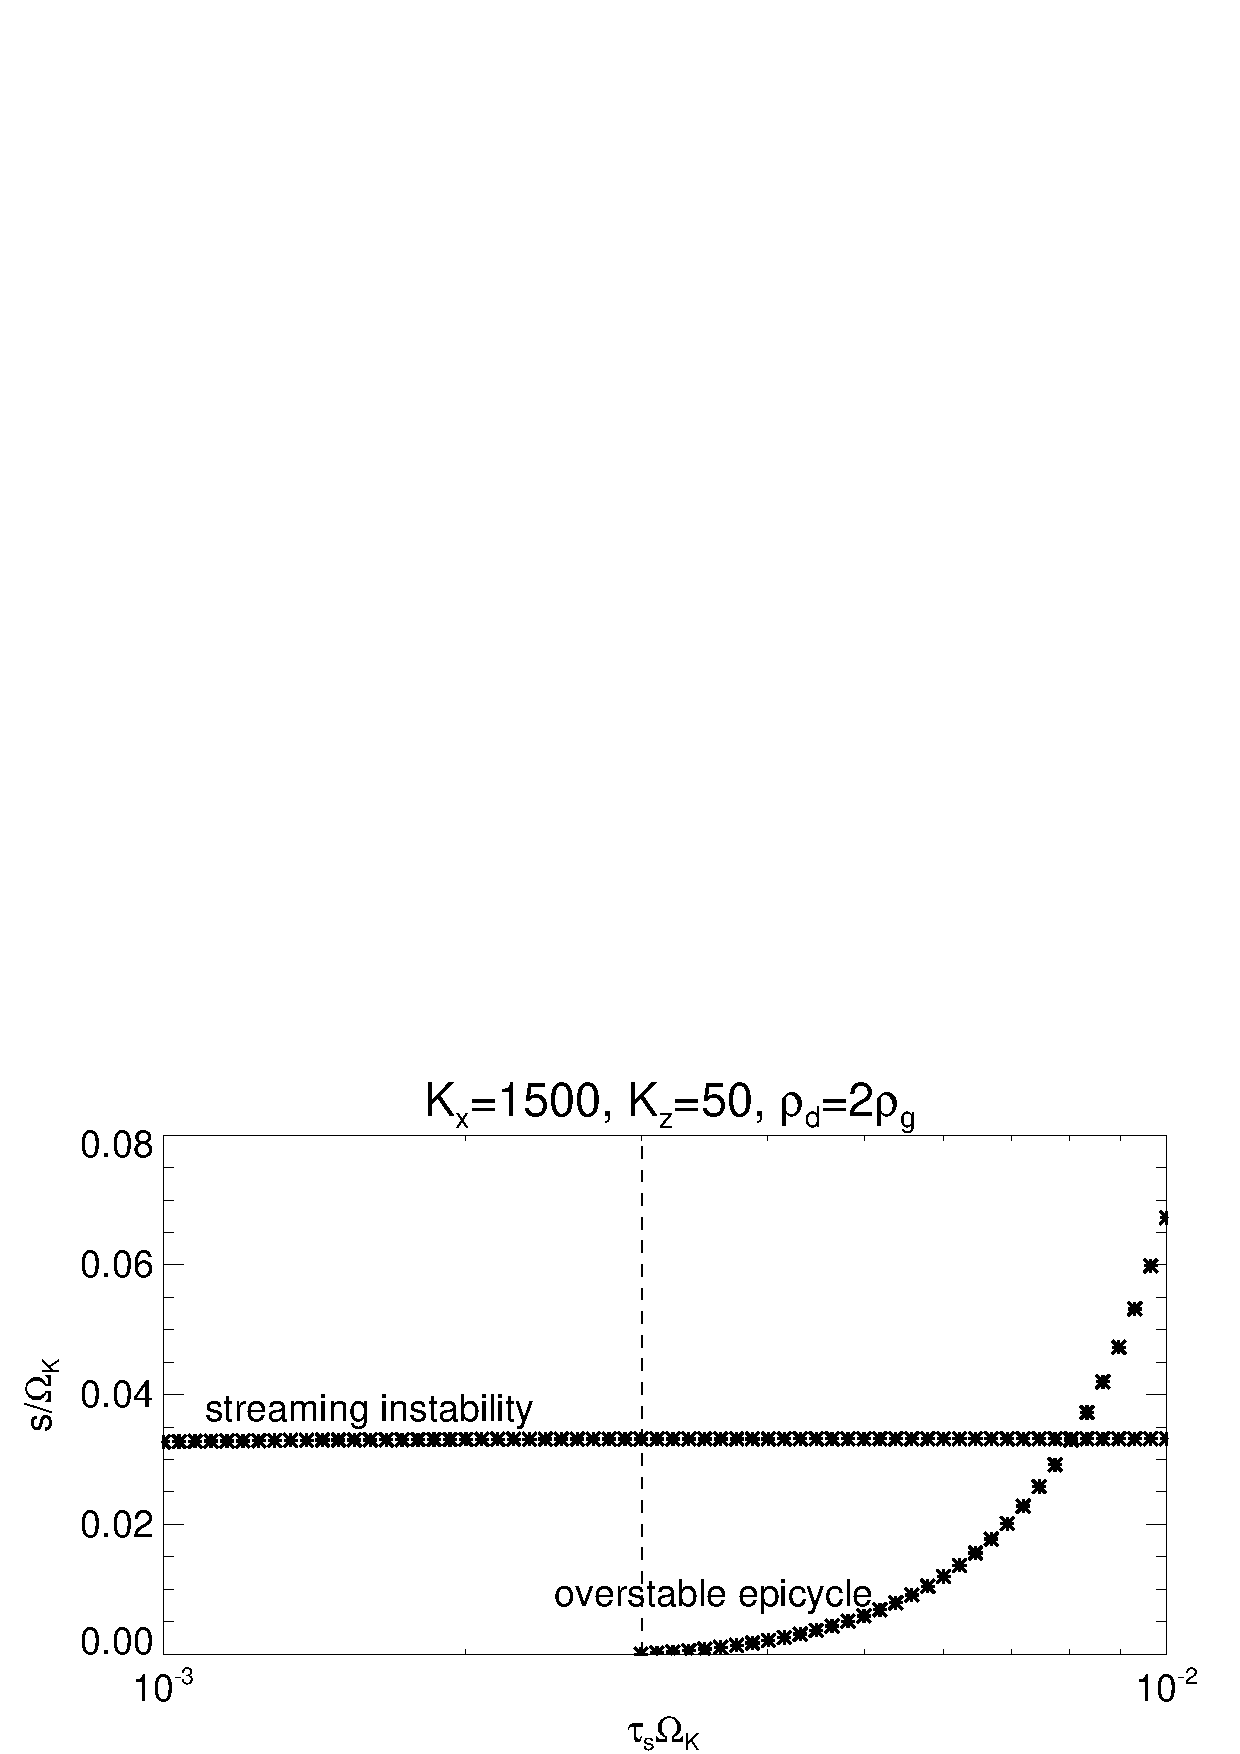
\includegraphics[width=\linewidth]{figures/streaming3}
%   \caption{Growth rates of dust-drag instabilities with fixed radial
%     wavenumber and dust-to-gas ratio, as a
%     function of stopping time at fixed vertical wavenumber. The
%     vertical dashed line correspond to the minimum stopping time for
%     growth of the dusty epicycle, given by
%     Eq. \protect\ref{epi_grow_criterion}. \label{dusty_growth2}
%   }
% \end{figure}

% These calculations suggest that in a realistic 3D dusty disk where
% vertical motions are allowed, the classic streaming
% instability is dominant because there exists $K_z$ values for which it
% dominates. This also renders the uncertainties in the  
% approximations used to describe the dusty epicycle modes
% irrelevant. On the other hand, the one-fluid framework can capture the
% streaming instability in the appropriate limit, as seen in Table
% \ref{si_compare}. 




%For small growth rates the real frequency $|\omega| =  
%O(\kappa)$, so these are overstable epicycles. 

%We finally note that Eq. \ref{epi_overs1}---\ref{epi_overs2} 
%admit pure oscillations with $s \equiv 0$, $\omega = 
%\pm\kappa$ if 
%\begin{align}
%  \tstop = \frac{\kappa}{k_x\left|F_r\right|}. 
%\end{align}
%This is the condition for marginal stability.  

% However, retaining all the terms (but still in the incompressible
% limit) can yield instability, as follows. Eq. \ref{kz_zero_si} admit
% pure oscillations with $\sigma = -\omega$ when 
% \begin{align*}
%   \omega &= \pm \kappa, \\
%   \tstop & = \frac{\omega}{ k _x F_r }
%          \equiv t_{\mathrm{s}0}.
% \end{align*} 
% Since $\tstop\geq 0$, we require $k_xF_r > 0$ if $\omega = \kappa$;
% and $k_xF_r < 0$ if $\omega = -\kappa$. For $k_x>0$ these marginally
% stable epicycles require radial pressure gradients decreasing and increasing
% outwards, respectively.  

%We require $\omega/k_xF_r> 0$  

% We now perturb about this state of marginal stability by writing
% $\sigma = \dd \sigma - \omega $ with $\dd\sigma = \ii\dd s -
% \dd\omega$, $\tstop = t_{\mathrm{s}0} +
% \dd\tstop $, and assume the $\dd$ quantities are small in
% magnitude. Then 
% \begin{align*} 
% \dd s = \frac{2\epsilon \kappa^2 }{1 +
%   4\epsilon^2 t_{\mathrm{s}0}^2\kappa^2}\dd \tstop. 
% \end{align*}
% Thus given $k_xF_r$, there exist growing modes 
% when the stopping time is slightly larger than
% $t_{\mathrm{s}0}$.  

% %{\bf note: several approx used}

% If we instead fix $\tstop$ and vary $k_xF_r$ about marginal stability,
% a similar exercise yields  
% \begin{align*} 
%   \dd s = \frac{\epsilon \tstop^3}{1 +
%   4\epsilon^2 \tstop^2 \kappa^2}\dd \left(k_x^2F_r^2\right).  
% \end{align*}
% Thus it is possible to destabilize the system by slightly increasing
% $|k_xF_r|>\kappa/ \tstop$ (i.e. shorter radial wavelengths and/or
% stronger pressure gradients).   

